\chapter{GSM}
\label{ch:gsm}
This chapter will give short overview of some important aspects of \gls{gsm}.
The first section will give a brief historical summary on the evolution of \gls{gsm} and how it came to be what it is today.
In section \ref{sec:network} the system architecture and its components as well as protocol basics will be explained that are essential to understand how an IMSI-catcher operates.
Section \ref{sec:catcher} will describe how an IMSI-catcher works and how it differs from the system components it replaces.
 
\section{A Historical Perspective}
The acronym GSM was originally derived fom \emph{Group Sp\'{e}ciale Mobile}.
This committee was part of the \gls{cept} 1982, with the task of developing a pan-Eurpean digital cellular mobile radio standard in the 900MHz range.
1986 the frequency range was officially licensed.
The foundation of this task group was a direct answer to the development of independent and incompatible analog radio networks during the 80's.
Examples of such networks were the C-Netz in Germany the \gls{tacs} in the UK or \gls{nmt} in Scandinavia.

In 1987 the committee submitted the basic parameters of GSM in February. 
Not far after, in September, the \gls{MoU} was signed in Copenhagen by 15 members of 13 Countries that were dedicated to deploy GSM in their respective countries.
This agreement was the basis for allowing international operation of mobile stations, using the interfaces agreed upon earlier that year.
\gls{cept} itself was around since 1959 and the member founded the \gls{etsi} in 1988.
In the same year the committee submitted the first detailed specification for the new communications standard.
The acronym was reinterpreted in 1991, after the committee became a part of the \gls{etsi} in 1989 to \emph{Global System for Mobile Communications}.
In the very same year the specifications for \gls{dcs1800} were also submitted.
These were essentially the same specifications, translated in the 1800MHz range and the foundation for the USA's 1900MHz band.
Under the umbrella of the \gls{etsi}, many \glspl{stc} began to work on different aspects of mobile communication, like network aspects (SMG 03) or security aspects (SMG 10).
SMG 05 dealt with future networks and especially with UMTS specifications, which eventually became an independent body inside the \gls{etsi}.

In 1992 many European countries had operational mobile telephone networks.
These networks were a huge success, and as soon as 1993 they already counted more than one million subscribers \cite{GSM2009}.
Also many networks on different frequency bands (900MHz, 1800MHz, 1900MHz) were started outside Europe in countries like the US or Australia, with Telstra as the first non European provider.
The rapid growth of mobile subscribers worldwide until today can be seen in figure \ref{fig:gsm_growth}.
Three of the main reasons for this rapid growth are explained by Heine \cite{protocols1999} as:
\begin{itemize}
	\item Liberalization of the mobile market in Europe, which allowed for competition and thus resulting in lower prices and enhanced development.
	\item Expertise within the Groupe Sp\'{e}ciale Mobile and their collaboration with industry.
	\item The lack of competitive technologies.
\end{itemize}

\begin{figure}
\centering
\begin{tikzpicture}
\begin{axis}[
	width=\textwidth,
	height=0.3\textheight,
	xlabel=Year, 
	ylabel=Subscribers,
	xticklabel style={/pgf/number format/1000 sep=}
	]
	\addplot [smooth,mark=*,blue] plot coordinates {
		(1994, 1e6)
		(1995, 10e6)
		(1996, 50e6)
		(1998, 100e6)
		(2001, 500e6)
		(2005, 1.5e9)
		(2007, 2.5e9)
		(2008, 3e9)
		(2009, 3.5e9)
		(2010, 3.7e9)
		(2011, 4e9)
	};
\end{axis}
\end{tikzpicture}
\caption{Growth of mobile GSM subscriptions. Compiled from \cite{GSM2009,GSM_history2011,GSM_stats2011}}
\label{fig:gsm_growth}
\end{figure}

\begin{figure}
\centering
\includegraphics[width=.5\textwidth]{../Images/3gpp.jpg}
\caption{The 3GPP Logo}
\end{figure}

In 1998 the \gls{3gpp} was founded by 5 organizational partners with the goal of standardization in mobile communications, with focus on developing specifications for a third generation mobile radio system.
These partners were \gls{arib}, \gls{etsi}, \gls{atis}, \gls{tta} and \gls{ttc}.
This focus was later expanded in the light of the \emph{International Mobile Communications-2000}-project \cite{3gpp_Proposal2000} of the \gls{itu} to 
\begin{itemize}
	\item Devolpment and maintainance of \gls{gsm} and \gls{gprs}, including \gls{edge}, which are standards for high speed packet oriented data transmission via \gls{gsm}.
	\item Development of a third generation mobile communication system on the basis of the old \gls{gsm} protocol. This standard is called \gls{umts}
	\item An IP based multimedia system.
\end{itemize}
Up to now, the \gls{3gpp} has enhanced mobile standards.
In 2005 the first \gls{hsdpa} network went online.
\gls{hsdpa} \cite{hsdpa} is a protocol that enables mobile users to download data with speeds up to 84Mbit/s since release 9.
\gls{hsupa} \cite{hsupa} is a related protocol in the \gls{hspa} family that provides similar high speed functionality for uploading data.
These and other specification are published on the \gls{3gpp} website\footnote{\url{http://www.3gpp.org/}}.

\section{The GSM Network}
\label{sec:network}

The \gls{gsm} network is a distributed, star shaped network type that is built on top of existing telephony infrastructure to additionally connect mobile users.
The telephony network is not only used to connect mobile subscribers to landline phones, but also to connect the different components of the mobile network.
The main components of a \gls{gsm} network can be seen in figure \ref{fig:gsm_network} as well as the interfaces that are used to connect them.
\begin{figure}
\caption{The main components of a GSM network.}
\label{fig:gsm_network}
\end{figure}
There are different notions of how to distribute these components into functional entities.
In the following the classification of \cite{kommsys2006} will be used.
It describes the main parts as:
\begin{itemize}
	\item \gls{bss}: this part is also called radio network and thus contains all the technology necessary for connecting mobile subscribers to the telephony network and routing their calls. 
	These calls originate from the \gls{ms} that will be explained in section \ref{sec:ms}, and travel over the air interface to the receiver stations for further processing.
	The air interface or $U_m$ interface will be explained in section \ref{sec:Um}, whereas the rest of the subsystem will be argued in section \ref{sec:bss}.
	\item \gls{nss}: the core network, as it is sometimes called, consists of several entities that are used to establish and route a connection.
	This is not only limited to calls within the provider's network but also into other provider's networks or the \gls{pstn}.
	The databases that contain subscriber information and location information for connected users are also located here, thus this is the place where mobility management is handled.
	\item \gls{in}: this part of the network augments the core network with \gls{vas} \cite{ITU1200}.
	In order to provide extra functionality the \gls{in} consists of several \gls{scp} databases.
	Some of the most used services are in fact services of the \gls{in} and not core services.
	Examples are prepaid cards, home areas\footnote{This service defines a geographical area, in which lower rates are calculated for mobile calls.} or telephone number portability.
\end{itemize}
Other sources define the \gls{oms} \cite{GSM2009} or limit the \gls{bss} entity to the provider part and define an additional entity for the \gls{ms} \cite{overview1994, overview1996}.
The three subsystems as well as the \gls{ms} will now be discussed in greater detail.

\subsection{Mobile Station}
\label{sec:ms}
With the advent of portable microprocessors in the 80's mobile phones became possible.
Advance in technology up to today yielded smaller mobile phones with more functionality year by year to a point where not the technology itself was the limiting factor for size, but the user interface, \eg button and display sizes.
Figure \ref{fig:phones} shows the evolution of the mobile phone over the last decades.
\begin{figure}
\caption{Evolution of mobile phones over the last decades.}
\label{fig:phones}
\end{figure}
What hasn't changed is the basic distinction between \gls{me} and \gls{sim}, the parts of which a \gls{ms} consists.

It is hard to deliver a consistent definition for what a \gls{me} is.
GSM Recommendation 02.07 \cite{GSM0207} summarizes the mandatory and optional features of a \gls{ms}.
Some of the most important mandatory features are \cite{protocols1999}:
\begin{itemize}
	\item \gls{dtmf} signaling capability.
	\item \gls{sms} capability.
	\item The cyphering algorithms A5/1 and A5/2 need to be implemented. 
	These are discussed in detail in section \ref{sec:nss}.
	\item Display capability for short messages and dialed numbers, as well as available \gls{plmn}s.
	\item Capable of doing emergency calls without \gls{sim} card.
	\item Machine fixed \gls{imei}.
	In a strict sense, this disqualifies many modern mobile phones, since the \gls{imei} is not fixed onto the device itself but is rather part of the software or firmware respectively.
	Tools like \emph{ZiPhone}\footnote{\url{http://www.ziphone.org/}} for iOS devices\footnote{\url{http://www.apple.com/ios/}}, especially iPhone, can change this supposedly unchangeable identifier.
\end{itemize}

The range of devices complying to these specifications is rather large, so categorizing can be challenging.
The intuitive approach would be to establish buckets by device type, but there are so many different devices as well as hybrid devices out there that this approach would not only be impracticable, but also too ambiguous.
Does a smartphone belong into the same category as a \gls{pda} or in the category of basic mobile phones; and what would a basic mobile phone be?

Another way to categorize different \gls{me}s is by supported frequency band and power class rating according to GSM  05.05\cite{GSM0505}.
Most mobile phones and smartphones belong to power class 4 and 5, which are for handheld devices.
Class 4 devices have and output of 2/33 W/dBm and class 5 0.8/29 W/dBm.
Classes with higher output are typically installed devices, \eg in cars.
These classes differ for the different frequency bands, since output needed in higher frequency bands (1800/1900 MHz) is less compared to the 900MHz band.
The supported band is also common category, since it describes in which countries a mobile phone can be used.
However it is more common nowadays that \gls{me} supports two bands or even all three bands.
These are called dual-band and tri-band devices respectively.

As the name suggests, the \gls{sim} card is essentially a data storage that holds user specific data.
This separation is interesting for the GSM user since it allows him/her to exchange the \gls{me} without having to contact the provider.
Thus it can be used on different frequency bands and is one of the preconditions for roaming.
The \gls{sim} card can either be in plug-in format or ID-1 SIM format which is normally used for telephone cards, credit cards or car installed \gls{me}.
The plug-in format is also called ID-000 and can be found in ISO/IEC 7810\cite{ISO7810}.

The most important information stored on a \gls{sim} card are the \gls{imsi} and the \gls{ki}.
A subset of other parameters stored on the \gls{eeprom}of the card can be seen in Table \ref{tab:simdata}.

\begin{table}
\centering
\begin{tabular}{@{}l>{\raggedright\arraybackslash}p{.8\textwidth}@{}}
\toprule
Parameter		&Description\\
\midrule
\multicolumn{2}{l}{Security Related}\\
\midrule
A3/A8			&Algorithms required for authentication and generation of the session key\\
Ki				&Secret key\\
Kc				&Session key, generated from a random number and Ki vie A8\\
PIN				&Secret numeric password to use a SIM card\\
PUK				&Secret numeric password to unlock the SIM card\\
\midrule
\multicolumn{2}{l}{Subscriber Data}\\
\midrule
IMSI			&Subscriber identification\\
MSISDN			&Telephone number\\
\midrule
\multicolumn{2}{l}{Network Related}\\
\midrule
LAI				&Identifier of the current location area\\
TMSI			&Temporary IMSI\\
Home PLMN		&Multiple entries to identify the home PLMN\\
\bottomrule
\end{tabular}
\caption{Subset of data stored on a SIM card. Adopted from \cite{protocols1999}}
\label{tab:simdata}
\end{table}

This key is used to generate the \gls{kc}, as will be explained in Section \ref{sec:nss}.
Most of this data, although not the security relevant \gls{ki} can be read via a USB \gls{sim} card reader, which can be bought for around \$10 on the web.
Since \gls{ki} never leaves the card, \gls{kc} has to be dynamically generated on the card.
This can be done since the card itself has a microprocessor that manages the security relevant data.
Key functions, like running the GSM key algorithm, verifying a \gls{pin} or reading a file can be accessed through the microprocessor via a communication protocol.
A brief description of the protocol and functionalities can be found in \cite{kommsys2006}.

\begin{figure}
\centering
\caption{Structure of the IMSI.}
\label{fig:IMSI}
\end{figure}

The \gls{imsi} as described in GSM 23.003\cite{GSM23003} uniquely identifies a subscriber.
The structure can be see in Figure \ref{fig:IMSI}.
It has at most 15 digits and is divided into three parts, \gls{mcc},\gls{mnc} and \gls{msin}, of which only the last part is the personal identification number of the subscriber.
The first two are also called \gls{hni}.
The three digit \gls{mcc} describes the country code, the area of domicile of the mobile subscriber.
The \gls{mnc} is an identification number for the home \gls{plmn}.
This can either have two or three digits depending on the \gls{mcc}.
It is not recommended by the specification and thus not defined to mix two and three digit \gls{mnc}s for a single \gls{mcc}.
These country codes are assigned by the \gls{itu} in ITU E.212\cite{ITU212}.
An excerpt can be found in Table \ref{tab:countrycodes}.
The third part, the \gls{msin} is a number consisting of up to ten digits, which is used for authentication of the mobile subscriber against his provider.
\gls{mnc} and \gls{msin} together are called \gls{nmsi}.
\begin{table}
\centering
\subtable{
\begin{tabular}{ll}
\toprule
Country		&MCC\\
\midrule
Germany		&262\\
France		&208\\
USA			&310 - 316\\
UK			&234 - 235\\
Switzerland	&228\\
Austria		&232\\
Poland		&260\\
\bottomrule
\end{tabular}
}
\hspace{.5cm}
\subtable{
\begin{tabular}{lll}
\toprule
Provider	&Country		&MNC\\
\midrule
T-Mobile	&Germany		&01, 06(R)\\
Vodafone	&Germany		&02, 04(R), 09(R)\\
E-Plus		&Germany		&03, 05(R), 77(T)\\
$O_2$		&Germany		&07, 08(R), 11(R)\\
Orange		&France			&00, 01, 02\\
Swisscom	&Switzerland	&01\\
A1			&Austria		&01, 09\\
\bottomrule
\end{tabular}
}
\caption{Mobile Country and Network Codes. (R) denotes that the MCC is reserved but not operational as of yet, whereas (T) denotes a operational test network.}
\label{tab:countrycodes}
\end{table}

\subsection{Base Station Subsystem}
\label{sec:bss}
The \gls{bss} is the part of the network that provides the hard- and software for physically connecting \glspl{ms} to the providers network.
Its main components are the \gls{bsc}, the \gls{bts} and the \gls{trau}.
Connecting of a mobile subscriber works via radio, which is why this subsystem is sometimes also called the radio network \cite{kommsys2006}.
Inside the radio network of a certain area, there is one \gls{bsc} that connects to multiple \gls{bts} and one \gls{trau}.
While the Transceiver station act as receiver for radio signals the controller coordinates the different receivers and relays the incoming signals  to the core network.
Since signals inside the core network are transmitted at other rates than in the radio network, rates need to be adapted, which is done by the \gls{trau}.

\subsubsection{The Cellular Principle}
\subsubsection{Baste Station Controller}
\subsubsection{Base Transceiver Station}
\subsubsection{Frequencies}
\subsubsection{Transcoding rate and Adaption Unit}

\subsection{Network Subsystem}
\label{sec:nss}
The most important task of the \gls{nss} or Network Switching Subsystem is to establish connections and route calls between different locations.
This is done by so called \gls{msc}, that can route a call either to another \gls{msc}, into the \gls{pstn} or another provider's network.
Apart from routing, the \gls{nss} also provides the means to administer subscribers inside the network.
Facilities to support this task are the \gls{hlr}, the \gls{vlr}, the \gls{eir} as well as the \gls{ac} that will now be described in further detail.
The \gls{smsc} is also part of this subsystem handling text messages.
A possible arrangement of these components is displayed in Figure \ref{fig:gsm_network}.

\subsubsection{Mobile Switching Center}
The \gls{msc} is the component that does the actual routing of calls and is thus the core component of the \gls{nss}.
Thus it basically works like any other \gls{isdn} exchange device with additional functionality to manage mobility
Since it would be the amount of signalling inside a \gls{plmn} would be far to big for a single \gls{msc}, there is one for every \gls{la}.
Amongst others its most important tasks are \gls{cc} and Mobility Management.

\gls{cc} entrails registration when the subscriber connects to the network as well as routing the calls or text messages from one registered subscriber to another. 
This routing can include transmitting calls to landlines or to networks of other providers.
\glspl{msc} that bind the provider's networks to other provider's networks or the \gls{pstn} are called Gateway \glspl{msc}.

The above part is also true for pure landline switching centres.
What sets a mobile switching centre apart is called Mobility Management.
Since the participants can freely move around in the network  and thus cannot be identified the same way as a fixed landline participant, authentication before using the offered services is important.
Another consequence of mobility is, that the network has to keep track of where a subscriber is and through which \gls{msc} it can be reached.
This is done via  Location Updates.
Also during calls if the subscriber leaves the respective service area of the switching centre, then the call needs to be transferred without being interrupted.
A procedure called Handover achieves just that.

For this central role to work it is necessary to be connected to all the other components of the \gls{nss}.
This is done via different connectors called Interfaces.
A brief description of what the different interfaces in a GSM network are and what their respective function is can be seen in Table \ref{tab:interfaces}.

\begin{table}
\centering
\begin{tabular}{lll}
\toprule
Name			&Between					&Function\\
\midrule
$A$				&MSC $\leftrightarrow$ BSS	&BSS management data for Mobility Management\\
				&							&and Call Control\\
$B$				&MSC $\leftrightarrow$ VLR	&MSC receives data about MSs in the current area\\
				&							& and sends data from Location Updates\\
$C$				&MSC $\leftrightarrow$ HLR	&MSC can request routing data during call setup\\
				&							&and send \eg charging information\\
$D$				&HLR $\leftrightarrow$ VLR	&Exchange of location-dependent subscriber data\\
				&							&and updating the HLR (MSRN \etc)\\
$E$				&MSC $\leftrightarrow$ MSC	&Executing a Handover when subscriber changes\\
				&							&to a new MSC\\
$F$				&MSC $\leftrightarrow$ EIR	&Checking white-/grey- and blacklists before\\
				&							&giving access to the network\\
\midrule
$A_\text{bis}$	&BSC $\leftrightarrow$ BTS	&BSC receives data from MS via the BTS\\
$U_m$			&BTS $\leftrightarrow$ MS	&Registration procedure, call data \etc as well\\
				&							&as broadcast information about the network\\
				&							&and the base station\\
\bottomrule
\end{tabular}
\caption{Interfaces inside the core network (upper part) and the radio network (lower part)}
\label{tab:interfaces}
\end{table}

\subsubsection{Home Location Register}
The \gls{hlr} is the central database in which all personal subscriber related data is stored.
The entries can be divided into two classes, permanent administrative and temporary data.
Part of this administrative data is which services a subscriber has access to and which are prohibited (\eg roaming in certain networks).
The data itself is indexed with the customer's \gls{imsi}, to which multiple telephone numbers can be registered.
Since these \glspl{msisdn} are independent from the \gls{imsi} a subscriber can change his telephone number and thus also move the telephone number along should he/she decide to switch to a new provider.
Basic services that access is stored for in the \gls{hlr} are amongst others the ability to receive and send telephone calls, use data services or send text messages.
Additional services, called Supplementary Services like call forwarding or display of phone numbers during calls can also be set or unset in this database.
It is up to the provider if these services are available freely or bound to a fee.
The temporary data enfolds the current \gls{vlr} and \gls{msc} address as well as the \gls{msrn} which is essentially a temporary location dependent ISDN number.

\subsubsection{Visitor Location Register}
As can be seen in Figure \ref{fig:gsm_network} there can be multiple \glspl{vlr}, one for each area in a network.
These registers can be seen as caches for data located in the \gls{hlr}.
Thus their are intended to reduce signalling between the \gls{msc} and the \gls{hlr}.
Each time a subscriber enters a new area, that is serviced by a new \gls{msc}, data for this subscriber is transferred to the respective \gls{vlr} from the \gls{hlr}.
Such data includes the \gls{imsi} and the \gls{msisdn} as well as authentication data and information on which services are available to that particular subscriber.
Additionally the subscriber is assigned a temporary \gls{imsi}, called \gls{tmsi} and information in which \gls{la} the \gls{ms} was registered last.
In this way the regular \gls{imsi} is not used and can thus not be harvested by tapping into the radio channel.
While it is possible to operate the \gls{vlr} as a standalone entity, in most cases it is implemented as a software component of the individual \gls{msc}.

\subsubsection{Equipment Identification Register}
The \gls{eir} is a database that contains the \glspl{imei} of registered \glspl{ms}.
It is used to determine whether a particular \gls{ms} is allowed to participate in communications.
For that purpose a white, a grey and a black list are used.
\glspl{imei} on the white list are allowed, while equipment that is grey-listed will be checked.
The blacklist is used to refuse access to \eg stolen equipment that has been reported to the provider.
In Germany only the providers Vodafone and E-Plus support blacklisting of \glspl{imei}\cite{blacklisting}.
Different companies like Airwide Solutions (now aquired by Manivir)\footnote{\url{http://www.mavenir.com/}} offer centralised lists for providers in their \glspl{ceir}.

\begin{figure}
\centering
\caption{Authentication procedure}
\label{fig:authentication}
\end{figure}
\subsubsection{Authentication Center}
The \gls{ac} is the network component responsible for authenticating mobile subscribers.
It is a part of the \gls{hlr} and the only place, apart form the customer's \gls{sim} card where the secret key \gls{ki} is stored.
The authentication is not only done once when the subscriber connects to the network, but rather on many occasions \eg the start of a call or other significant events to avoid misuse by a third party.
This authentication routine is a key based challenge-response procedure outlined in Figure \ref{fig:authentication}.
The steps of the procedure can be summarized as follows:
\begin{enumerate}
	\item User connects to the network or triggers an event that needs authentication at the \gls{msc}.
 	
 	In the first case the \gls{imsi} is part of the authentication request and the \gls{ac} starts with searching for the corresponding \gls{ki} and authentication algorithm A3.
	An authentication triplet is build using \gls{ki} which consists of the components:
	\begin{itemize}
		\item RAND: a 128 bit random number.
		\item SRES: a 32 bit number called signed response, which is generated by A3 with \gls{ki} and RAND as inputs.
		\item Kc: the ciphering key that is used to cypher the data during transmission.
		It is also generated with \gls{ki} and RAND.
	\end{itemize}
	To save signalling bandwidth, usually more than one authentication triplet is generated and returned to the \gls{msc} by the \gls{ac}.
	It should be noted that, since a separate cyphering key is used, the secret key never leaves the \gls{ac}.
	
	In the second case, either a previously generated authentication triplet is used, or new authentication triplets are requested.
	\item RAND is transmitted to the \gls{ms} by the \gls{msc} where the signed response SRES* is created by the \gls{sim} card using A3, \gls{ki} and RAND.
	
	\item An authentication response containing SRES* is sent back to the \gls{msc}.
	
	\item If SRES and SRES* are the same, the subscriber is authenticated.
\end{enumerate}

Remarkable properties of this procedure are that by using a cyphering key that is generated by a random number and a secret key, the secret key itself never leaves the \gls{ac}.
Apart from that the use of a random number prevents replay attacks on SRES.
It should also be noted that this way of authenticating only works for authenticating the subscriber to the network.
It is a one way authentication.
The subscriber needs to trust the network.
This is a design flaw that IMSI-Catchers use to lure \gls{ms} into their fake network.
In \gls{umts} networks that flaw was fixed and the authentication procedure was made mutual.

\subsection{Intelligent Network}
The two subsystems above are necessary for the correct operation of a \gls{gsm} network.
While the \gls{in} is not essential for operation, all providers offer additional services that need additional logic and databases.
These databases are called \gls{scp} databases and are one of three possible \gls{ss7} nodes.
They can influence the build-up of a connection or modify parameters for that specific connection.

Two of the most common services offered are \gls{lbs} and prepaid services.
An Example for a well known \gls{lbs} that is provided by the \gls{in} is a dynamic calling rate service.
If the mobile subscriber is in a specific geographical area, the \gls{scp} can modify the Billing Record to lower the calling rates.
This is known as home-zone.
If a mobile subscriber uses a prepaid service, an account is created for this subscriber that can be topped up.
Afterwards calls and text messaged use up the money on that account.
This is an alternative to a monthly bill and attracted many customers since its advent in the mid 90's.
For this service the \gls{scp} needs to constantly update the money on the account during calls and when text messages are sent.

Since these services were defined as additional and thus no specification existed, they evolved into vendor specific proprietary networks, that were not interoperable.
To standardize these services, \gls{3gpp} and \gls{etsi} defined the \gls{camel} protocol in TS 23.078\cite{GSM23078}.
\gls{camel} specifies a protocol much like \gls{http} that regulates how the different components of a \gls{gsm} network exchange information.
As such it is not an application itself but rather a framework to build vendor independent, portable services.

\section{The $U_m$ Interface}
\label{sec:Um}
\subsection{Layers}
\subsection{The Radio Channel}
\subsection{Logical Channels}
\section{IMSI-Catcher}
\label{sec:catcher}
\subsection{Mode of Operation}
\subsection{Possible Attacks}
\subsection{Law situation in Germany}
%germany not plagued by terrorism
%response to 9/11: overreaction (Luftschutzgesetz)
%no definition for terror in german law
%preventive meassures taken
%government can influence prosecution

%---- procedural law ------
%terrorists/criminals switch mobile phone/sim cards often
%imsi-catcher: identification to apply telephone surveillance, whereabouts for arrest warrant, no other purpose allowed
%prior authorization by a judge (legislative power) or prosecutor (executive power) in case of emergency ----> revoked
%2004: no electronic surveillance in private premises HOWEVER for data needed for criminal cundoct allowed
%sacrifice of personal rights for crime surveillance
%threshold for elecronic surveillance is VERY low when the word terrorism or serious crimes bumps up
%police needs to show certain evidence underpinning a suspicion that such a criminal act was committed, attempted or prepared
%evidence from agents that is not transparent

%"Electronic surveillance, it seems, is no
%longer governed by questions of legitimacy, but solely by the question of practi-
%cality. Every method that is practical, will be used by police and agencies.37
%Often enough the courts have given up any serious control of investigation
%methods"
%See U. Eisenberg and T. Singelnstein, ‘Zur Unzulassigkeit der heimlichen Ortung per ‘‘stiller
%SMS’’’, 25 Neue Zeitschrift fur Strafrecht (2005) 62, at 67.

%easier share of sensitive information between police/intelligence/prosecution
%similar examples for other areas like surrender of citizens



